\chapter{Design}
\section{Workflow}
Three workflows have been defined within this section which are made to be modular allowing for interchangeability and independence from each other. These can be implemented using a plethora of technologies available to a developer.
% % % % % % % % % % % % % % % % % % % % % % % % % % % % % % % % 
% % % % % % % % % % % % % % % % % % % % % % % % % % % % % % % % 
\subsection{Application Module}
\begin{figure}[H]
    \centering
    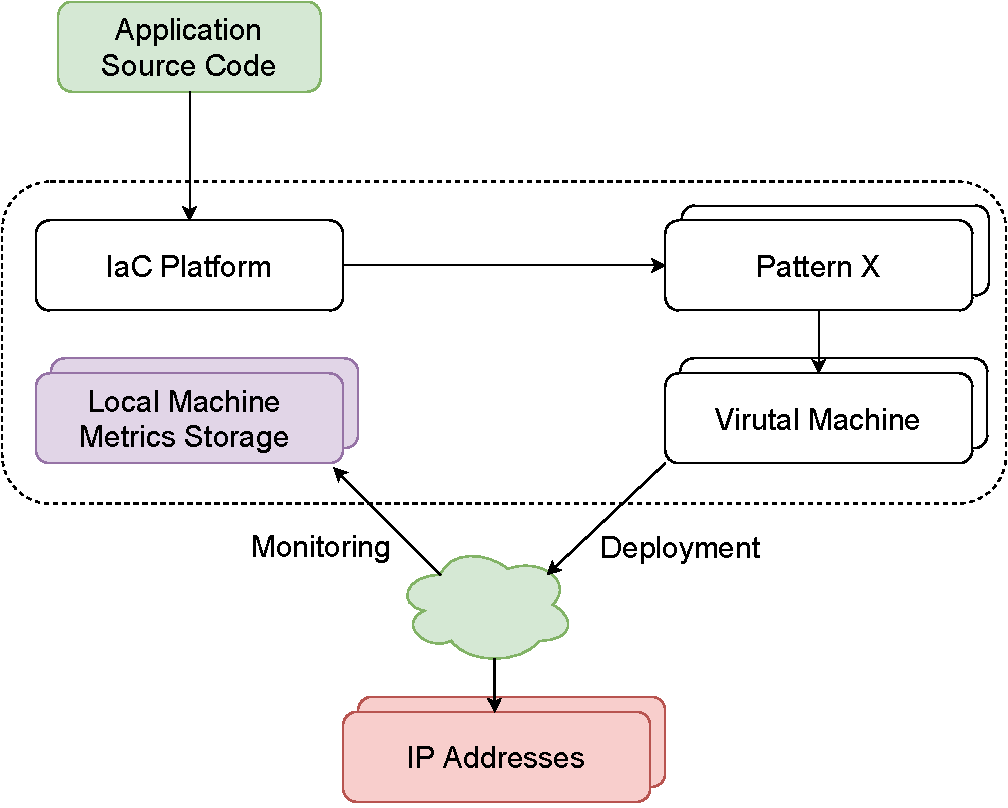
\includegraphics[width=0.7\linewidth]{images/Modular_Application.pdf}
    \caption{Application flow using Pattern 1.}
\end{figure} 

As seen in Figure 4.1, the module accepts application source code, this is used by the IaC platform to create multiple virtual machines inside the chosen pattern within the cloud. Followed by an output of new host IP addresses, this stage can be called the creation stage. A modular design of such allows for the IaC platform to create multiple machines at a time, which can be used for executing multiple tests, helping in reducing time. Once the creation stage has been completed, the module is set to an ideal state. Followed by the creation of the load module and after a certain time the application module enters a destruction stage where it collects the machine metrics from the cloud provider storing them locally, followed up by clearing up all machines in the cloud. 
% % % % % % % % % % % % % % % % % % % % % % % % % % % % % % % % 
\subsection{Load Module}
\begin{figure}[H]
    \centering
    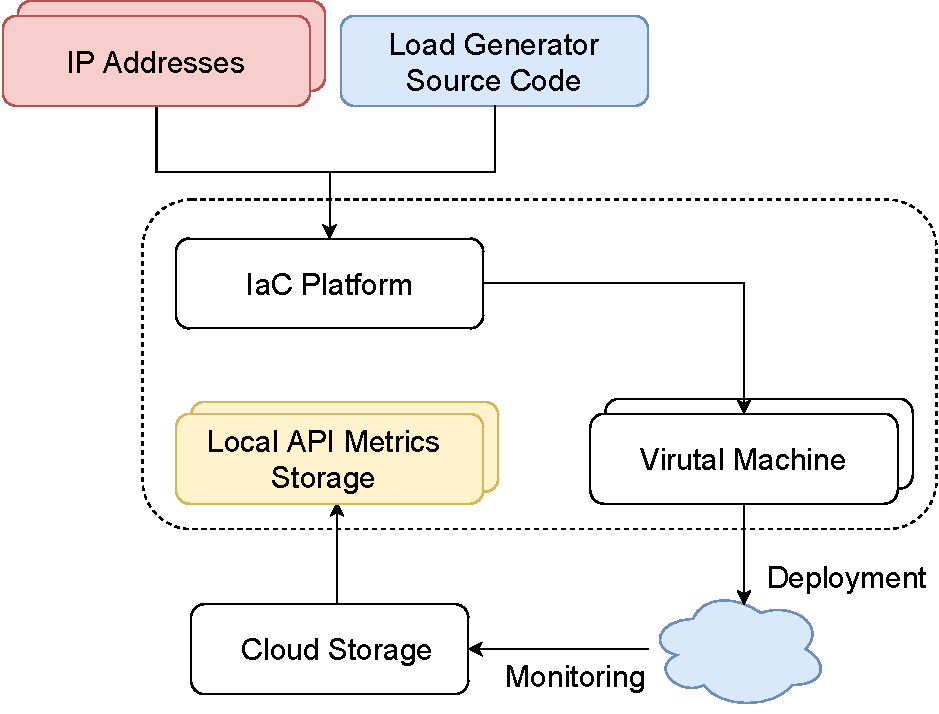
\includegraphics[width=0.7\linewidth]{images/modular_load.pdf}
    \caption{Load Generator flow using Pattern 1.}
\end{figure} 
As seen in Figure 4.2, the load module accepts a list of host IP addresses and the application's load generation source code. This is used by the IaC platform to create subsequent virtual machines to general load based on the IP addresses provided. This leads to the test machines sitting in a loading state where the application machines are simulated for performance testing. Once the load state has finished simulating the machines, the log files are stored to the cloud storage provided by the cloud provider, which is later downloaded locally, this is followed up by clearing up all machines in the cloud. 

% % % % % % % % % % % % % % % % % % % % % % % % % % % % % % % % 
\subsection{Analysis Module}
\begin{figure}[H]
    \centering
    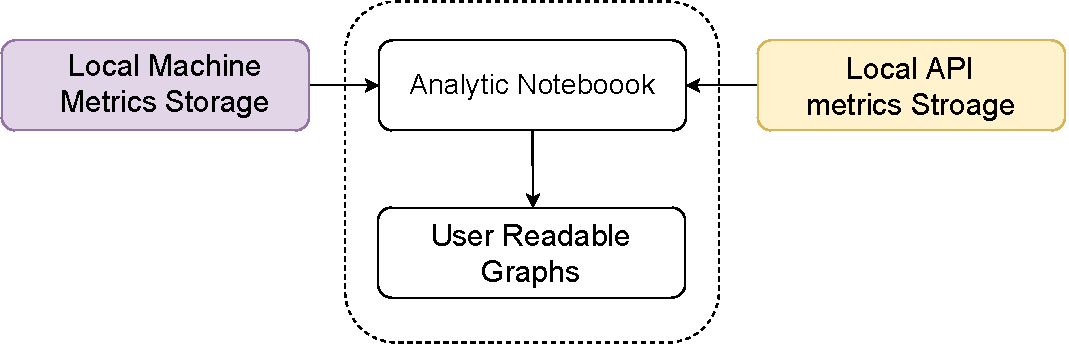
\includegraphics[width=0.5\linewidth]{images/Data Flow.pdf}
    \caption{Data flow using Pattern 1.}
\end{figure} 
The analysis module in figure 4.3, uses the machine metrics and load files generated from the above modules to create meaningful user readable graphs. 

\subsection{Lifetime Flow}
\begin{figure}[H]
    \centering
    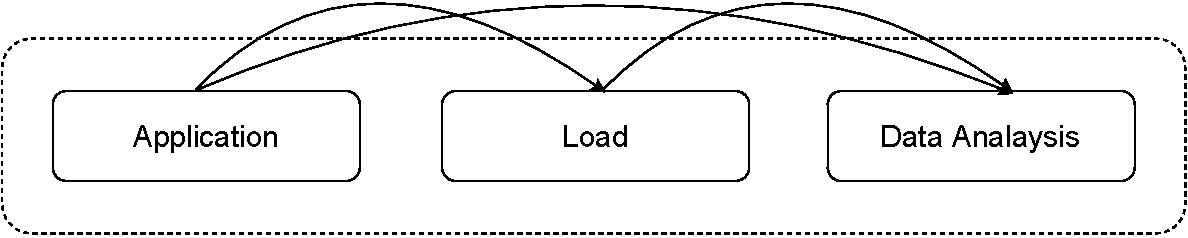
\includegraphics[width=0.5\linewidth]{images/Flow-Information.pdf}
    \caption{Flow of information between different modules.}
\end{figure} 
Figure 4.4 displays the flow of information between each module. 

\section{Experimental Design}



% The flow starts with a packaged microservice application, possibly stored on a version control system, where the source code for the application and load generator is kept separate from each other whilst also being easily accessible. 
% \\
% The source code follows two paths, controlled by the Main Script, where 
% \\
% \hspace*{6mm} \textbf{Path A} flows into the Infrastructure as a Code (IaC) platform which boots up a suitable virtual machine based on the requirements, such as deploying Pattern's one or two, which require modifications in the IaC script, once a machine is booted, the application can be hosted within the machine returning the Host's IP address with the application forwarded to the port address.
% \\
% \hspace*{6mm} \textbf{Path B} follows a similar path, however, skips out on the patterns, and is created after the application machine is hosted. Path A and B collide at this point, where B takes in the Host IP Address, and runs the load generator scripts for a certain amount of time, saving this data to the cloud provider so it can later be downloaded locally. 

% This is where the unit A's machine metrics are pulled from the provider and stored locally side by side to the API metrics. This concludes the use of both cloud machines and can be safely dropped. At the last stage of the workflow, both paths with the machine and API metrics flow into the analytical notebooks where data can be made sense of and compared to. 

